\section{Scaling of the Application}
\label{sec:Scaling_of_the_Application}
 Experiments were designed to test the scalability of the application. As mentioned in Section~\ref{sec:intro_scaling}, the application did not scale particularly well. Strong scaling experiments were conducted on both single node and multi-node hardware configurations.


\subsection{Experiment Set-up}
Scaling experiments were performed for the 'closest vector problem' using the C++ layer of the QNLP library. This involved encoding a set of binary vectors into a superposition of quantum states, adjusting the amplitude of each state proportionally to the Hamming distance between each state's binary vector and a test vector, followed by a measurement of the state. This was repeated a large number of times to generate a distribution of the measured states. The execution time for this experiment was measured using timing instrumentation. Strong scaling experiments were conducted by varying the number of processes used (compute resources) while maintaining a fixed total problem size (length of binary vector). Weak scaling experiments were not performed due to time constraints, but will be rigorously tested during the next phase of the project. Each individual experiment was run for $500$ iterations.

The reason that the pre-computation steps (involving the parsing of the corpus, tagging, and application of the distributed and compositional semantic algorithms) was not included in these scaling experiments was because they do not directly interact with the quantum simulator. It would be very difficult to find different corpus which would have a problem size that could be proportionally varied for the required range of compute resources needed for the scaling experiments. Furthermore, the pre-computation stage contributes to a relatively very small proportion of the total compute time of the application, and it's output is precisely the binary vectors that are being encoded into the superposition of states, thus the pre-computation can be ignored at this stage of the scaling experiments. If the run-time of the 'closest vector problem' implementation improves significantly, adding the pre-computation steps to the scaling performance analysis will be considered.

The ICHEC HPC cluster Kay was used for all experiments. Each compute node consists of $2\times 20$-core $2.4$ GHz Intel Xeon Gold $6148$ (Skylake) processors, $192$ GiB of RAM, a $400$ GiB local SSD for scratch space and a $100$ Gbit OmniPath network adaptor. This partition has a total of $336$ nodes consisting of $13440$ cores and $63$ TiB of distributed memory.

\subsection{Single Node Scaling}
\label{sec:single_node_scaling}
Scaling experiments were performed on a single compute node with $2^n$ processes for $n=0,1,2,3,4,5$ ($2^5 = 32$ which is the maximum power of $2$ that is below 40, the number of CPU's on a node, which is a constraint of the Intel\textregistered-QS). Strong scaling was conducted using a binary string length of 6 which implies a total of $2\times 6 + 2 = 14$ qubits were used during the computation. The plotted results of these experiments are shown in Figure~\ref{fig:scaling_single_node}. The full table of results are shown in Table~\ref{tab:scaling_results}.

From observing Figure~\ref{fig:scaling_single_node}, the application achieves near linear scaling for a smaller number of processes which begins to diverge as the number of processes increases. This is an expected result. Also, note that for a single process the execution time is $1903$ seconds, which decreases by an order of magnitude for $8$ or more processes. Thus, the application scales well on a single node for a relatively small problem size and increasing the number of processes has a significant effect on reducing the execution time.


\begin{figure}[htbp]
    \centering
    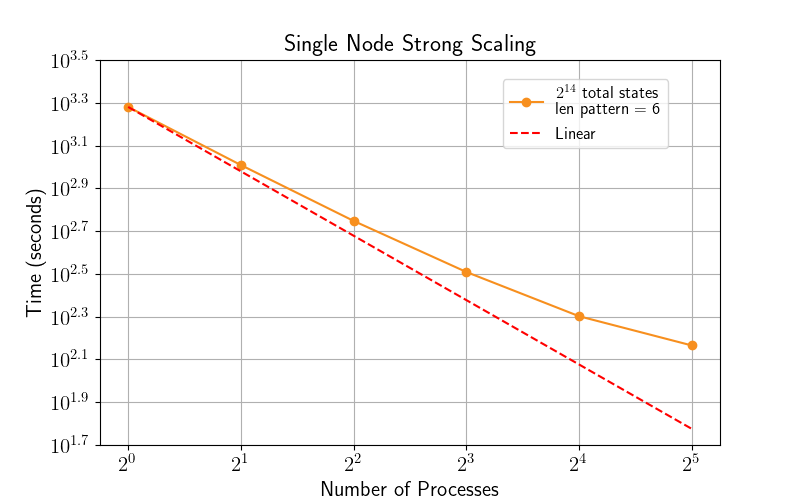
\includegraphics[width=0.95\textwidth]{Images/Scaling/Single_Node_Strong_binlen6.png}
    \caption{Scaling of the application for varying number of processes on a single node, each with one thread. The length of the binary string was $6$ which means a total of $14$ qubits were used. The linear scaling plot is shown in red.}
    \label{fig:scaling_single_node}
\end{figure}

\subsection{Multi-Node Scaling}
\label{sec:multi_node_scaling}
Scaling experiments were also performed for a varying number of processes per node on varying numbers of nodes. This was done to see the effect of MPI communication overhead across nodes as the number of nodes and subsequently processes were increased.

A single strong scaling experiment was conducted by fixing the number of processes per node and the problem size. The total number of processes was then increased by increasing the number of nodes used. This experiment was repeated for varying numbers of processes per node. The problem size was fixed, using a binary string length of $8$, which means the total number of qubits used was $2\times 8 + 2 = 18$. The number of nodes used was $1,2,4,8,16$ and $32$, each with $8,16$ and $32$ processes per node. The plotted results of these experiments are shown in Figure~\ref{fig:scaling_multi_node}. The complete list of results are shown in Table~\ref{tab:scaling_results}.

From observing Figure~\ref{fig:scaling_multi_node}, the application scales almost identically as the number of processes is increased but on different numbers of nodes (different numbers of processes per node). This indicates that inter-node MPI communication does not have a significant impact on the application's scaling for small to medium problem sizes. However, this will need to be tested for larger problem sizes that saturate a node's memory to fully determine. This is because for an experiment, each quantum state can fit in the cache simultaneously. 

The linear scaling for $8$ processes per node is shown in red. Comparing the scaling of each experiment to the linear scaling, the application scales almost linearly for smaller numbers of processes per node, but diverges as the number of processes increases. This is consistent with the observed results for a single node in Section~\ref{sec:single_node_scaling}. Note, for $32$ processes and greater, the execution time is at least an order of magnitude smaller than for $8$ processes. Thus, increasing the number of processes has a significant effect on reducing the execution time.

\begin{figure}[htbp]
    \centering
    \includegraphics[width=0.95\textwidth]{Images/Scaling/multi_node_scalingstrong.pdf}
    \caption{Scaling of the application for varying number of processes on multiple nodes, each with one thread. Every experiment had a fixed number of processes per node. The length of the binary string was $8$ which means a total of $18$ qubits were used. The linear scaling for $8$ processes per node is also shown in red.}
    \label{fig:scaling_multi_node}
\end{figure}

\subsection{Scaling Results}
Table~\ref{tab:scaling_results} details the results of all the scaling experiments conducted for this deliverable. The findings of these results have already been detailed in Sections~\ref{sec:single_node_scaling} and~\ref{sec:multi_node_scaling}. One further point to note about these results is the memory usage per node for the given problem sizes. The largest amount of memory used on a node was $2$MB in these experiments. This was for a binary length of $8$ on a single node. The available memory per node is $192$GB. Thus, the memory usage per node is under-utilised. However, as the number of qubits increases, the number of gate calls in the \textit{nCU} operation explodes, thus increasing the run-time significantly. This was tested for the experiments listed in Table~\ref{tab:scaling_results} using a binary length of $9$ (20 qubits), however these experiments scaled very poorly. Thus, for larger problem sizes, the application does not scale well. Further scaling experiments for larger problem sizes need to be conducted to observe the application's behaviour better. However, these will be conducted on the optimised \textit{nCU} implementation of the application which is expected to scale much better than the current version. The optimised version of the application is still expected to not scale too well due to the large number of gate calls that remain in the \textit{nCU} decomposition.

\begin{table}[h!]
\centering
    \begin{tabular}{||c|c|c|c|c|c|c|c||}
        \hline
        Nodes    &  Procs  &    Num   & Bin       &    Storage &    StoragePer   &    StoragePerNode    &    Time    \\
             &   PerNode  &   Procs    &   Len        &    PerNode  &    State     &    Temporary     &       \\
            &      &       &           &     (MB) &     (MB)    &     (MB)    &  (s)     \\         
        \hline
        \hline
         1   &   1   &   1   &   6   &     0.38    &   0.25    &   0.12500 &   1903    \\
         1   &   2   &   2   &   6   &     0.38    &   0.25    &   0.12500 &   1018    \\
         1   &   4   &   4   &   6   &     0.38    &   0.25    &   0.12500 &   558 \\
         1   &   8   &   8   &   6   &     0.38    &   0.25    &   0.12500 &   322 \\
         1   &   16  &   16  &   6   &     0.38    &   0.25    &   0.12500 &   200 \\
         1   &   32  &   32  &   6   &     0.38    &   0.25    &   0.12500 &   146 \\
         \hline
         1   &   32  &   32  &   8   &     6.00    &   4.00    &   2.00000 &   34856   \\
         2   &   32  &   64  &   8   &     3.00    &   2.00    &   1.00000 &   18852   \\
         4   &   32  &   128 &   8   &     1.50    &   1.00    &   0.50000 &   10868   \\
         8   &   32  &   256 &   8   &     0.75    &   0.50    &   0.25000 &   6663    \\
         16  &   32  &   512 &   8   &     0.38    &   0.25    &   0.12500 &   4562    \\
         32  &   32  &   1024    &   8   &     0.19    &   0.12    &   0.06250 &   3618    \\
         \hline
         1   &   16  &   16  &   8   &     6.00    &   4.00    &   2.00000 &   67360   \\
         2   &   16  &   32  &   8   &     3.00    &   2.00    &   1.00000 &   35058   \\
         4   &   16  &   64  &   8   &     1.50    &   1.00    &   0.50000 &   19022   \\
         8   &   16  &   128 &   8   &     0.75    &   0.50    &   0.25000 &   11020   \\
         16  &   16  &   256 &   8   &     0.38    &   0.25    &   0.12500 &   6624    \\
         32  &   16  &   512 &   8   &     0.19    &   0.12    &   0.06250 &   4743    \\
         \hline
         1   &   8   &   8   &   8   &     6.00    &   4.00    &   2.00000 &   131896  \\
         2   &   8   &   16  &   8   &     3.00    &   2.00    &   1.00000 &   67604   \\
         4   &   8   &   32  &   8   &     1.50    &   1.00    &   0.50000 &   35216   \\
         8   &   8   &   64  &   8   &     0.75    &   0.50    &   0.25000 &   19080   \\
         16  &   8   &   128 &   8   &     0.38    &   0.25    &   0.12500 &   10981   \\
         32  &   8   &   256 &   8   &     0.19    &   0.12    &   0.06250 &   6721    \\
        \hline
        \hline
    \end{tabular}
    \caption{Results of all scaling experiments shown in plots. Each individual experiment was run for $500$ iterations.}
    \label{tab:scaling_results}  
\end{table}


